\begin{reviewer}
This work developed a useful probabilistic framework to estimate the transient power and temperature variations of electronic system designs. The description is clear, and the organization is well.
\end{reviewer}
\begin{authors}
Thank you.
\end{authors}

\begin{reviewer}
A few of comments and suggestions are listed as follows.

\clabel{4}{1a}
The computational complexity of the proposed framework should be analyzed.
\end{reviewer}
\begin{authors}
The analysis of the time complexity of the framework is available.
It was not included in the manuscript as we tried to avoid those things that could not be explained clearly within the given space limit.
A clear explanation requires an in-depth discussion on the algorithmic structure of the proposed framework since the particularities of our implementation are important for the performance of the proposed approach.
In particular, a thorough analysis is needed to the parts of the algorithm that stay unchanged when the input changes.
These parts can and should be precomputed and stored so that their future use implies no additional computational costs; this is partially related to \cref{4}{2} regarding Sec.~VI-D.
Taking the received feedback into account, we have reconsidered our decision and have included in the revised manuscript a concise version of the analysis of the time complexity, given as follows.

All the statements below regarding certain aspects of PC expansions should be understood in the context of our implementation.
Recall that $\nprocs$, $\nnodes$, $\nsteps$, $\pcterms$, and $\qdorder$ are the numbers of processing elements, thermal nodes, time steps, polynomial terms, and quadrature points, respectively.
The construction of PC expansions is based on so-called non-intrusive spectral projections [Eldred, 2008] using quadrature rules.
The needed quadrature rule is determined solely by the intended PC expansion.
The structure of the intended PC expansion, \ie, everything except for the coefficients, is determined solely by the desired accuracy, \ie, $\pcorder$, and the parametrization of the problem in terms of independent variables, \ie, $\vZ(\o)$.
Therefore, any two problems that share $\vZ(\o)$ and $\pcorder$ have identical structures of PC expansions and identical quadrature rules.
To give an extreme example, suppose a dual-core platform has three uncertain parameters $\vU'(\o)$, and a 32-core platform has 33 uncertain parameters $\vU''(\o)$.
Then, if the model order reduction procedure leaves two beta variables $\vZ(\o)$ in both cases, the two problems are identical from the perspective of, say, the fourth-order PC, regardless of the input dynamic power profile.
Consequently, the preliminary work for a fix combination of $\vZ(\o)$ and $\pcorder$ should be done only once.
In particular, this means that, for a given electronic system and a given accuracy level, an unlimited number of dynamic power profiles can be analyzed at no extra effort.
This is especially advantageous for various optimization procedures, as we note in Sec.~VII.

Going deeper in detail, for each problem, we compute and store two matrices.
The first one is an $\pcterms \times \qdorder$ matrix, referred to as the projection matrix, which is used to compute the coefficient of a PC expansion by one matrix multiplication.
The second one is an $\pcterms \times \qdorder$ matrix, referred to as the evaluation matrix, which is used to evaluate a PC expansion at the quadrature nodes by one matrix multiplication.
Having said all above, we can now calculate the time complexity of the PC expansions computed inside the proposed framework.
As usual, the costs associated with other preliminary computations which are constant for a particular problem/platform, \eg, the construction of equivalent thermal RC circuits, are not included.

The iterative procedure in Eq.~7 traverses $\nsteps$ time steps.
Each step yields an $\nnodes \times \pcterms$ matrix that contains the coefficients of a PC expansion for temperature.
This matrix is the sum of two matrices corresponding to the two terms in Eq.~7.
The first matrix is based on the result from the previous iteration and is obtained by one multiplication of an $\nnodes \times \nnodes$ matrix with an $\nnodes \times \pcterms$ matrix.
The second matrix is computed by one multiplication of an $\nnodes \times \nprocs$ matrix with an $\nprocs \times \pcterms$ matrix, representing the coefficients of the current PC expansion for power.
So, the complexity of one step up to this point is $\O(\nprocs^2 \, \pcterms)$ since $\nnodes$ is typically proportional to $\nprocs$; for example, in the experimental results, $\nnodes = 4 \, \nprocs + 12$.
The calculation of the current PC expansion for power is composed of two stages: evaluation and projection.
At the first stage, the current PC expansion for temperature, that is, the one from the previous step, is evaluated at the quadrature nodes.
As mentioned earlier, this operation is one multiplication of an $\nprocs \times \pcterms$ matrix with the evaluation matrix; so, this operation is $\O(\nprocs \, \pcterms \, \qdorder)$.
Then, the power model is utilized to obtain an $\nprocs \times \qdorder$ matrix of power based on the evaluated temperature, \ie, an $\nprocs \times \qdorder$ matrix, and the assignments of the uncertain parameters with respect to the quadrature nodes, which is another $\nprocs \times \qdorder$ matrix.
This operation can be better viewed column-wise.
Denote the complexity of the computations associated with the power model for one pair of columns by $\O(\vP(\nprocs))$; hence, for $\qdorder$ columns, it is $\O(\qdorder \, \vP(\nprocs))$.
At the projection stage, the coefficients of the current PC expansion for power are calculated by one multiplication of the output of the power model, \ie, an $\nprocs \times \qdorder$ matrix, with the projection matrix; so, this operations is $\O(\nprocs \, \qdorder \, \pcterms)$, which is the same as the complexity of the evaluation stage.
The time complexity of one time step is then
\[
  \O(\nprocs^2 \, \pcterms + \nprocs \, \qdorder \, \pcterms + \qdorder \, \vP(\nprocs)).
\]
The first term can be dropped as $\nprocs$ is typically much smaller than $\qdorder$.
Taking into consideration all the time steps, we have
\[
  \O(\nsteps \, \nprocs \, \qdorder \, \pcterms + \nsteps \, \qdorder \, \vP(\nprocs)).
\]
The expression can be detailed even further by expanding $\pcterms$ and $\qdorder$.
For total-order polynomial spaces, the exact formula for $\pcterms$ is given in Eq.~5.
The limiting behavior of $\pcterms$ with respect to $\nvars$ is $\O(\nvars^\pcorder / \pcorder!)$.
For sparse grids, $\qdorder$ does not have such a closed-form formula and depends on the family of the quadrature rule utilized.
The limiting behavior of $\qdorder$ with respect to $\nvars$, however, has been extensively studied.
For example, for Gaussian quadratures, $\log(\qdorder)$ is $\O(\log(\nvars))$, which means that the dependency of $\qdorder$ on $\nvars$ is polynomial [Heiss, 2008].
In contrast, for full-tensor-product grids, this dependency is exponential.

\begin{actions}
  \action{The time complexity has been included in Sec.~V-D4.}
\end{actions}
\end{authors}

\begin{reviewer}
\clabel{4}{1b}
The authors also should compare the estimated stochastic power profiles provided by the proposed framework with those obtained by the MC simulations.
\end{reviewer}
\begin{authors}
Let us first note that the following discussion is partially included in our answer to \cref{2}{3}.

Despite the fact that the proposed framework covers both power and temperature, we initiated this work aiming at the quantification of temperature, not power \perse\ as it had already been addressed by other researchers.
In other words, our main focus was always on temperature.
Therefore, and also considering space limitations, the experimental results are primarily dedicated to temperature analysis, which makes the main contribution of our research.

Furthermore, power is an intermediate step towards temperature and, thus, resides closer to the sources of uncertainty in the chain of various transformations.
Therefore, the quantification of power is expected to be easier than the quantification of temperature, and any accuracy problems with respect to power are expected to eventually propagate to temperature.
Hence, the assessment of temperature allows us to implicitly draw reasonable conclusions with respect to power.

\begin{actions}
  \action{The absence of comparisons for power has been motivated in Sec.~VII.}
  \action{The power/temperature relation with respect to accuracy has been discussed in Sec.~VII.}
\end{actions}
\end{authors}

\begin{reviewer}
\clabel{4}{2}
In section VI.D, the authors mentioned that ``these points along with the corresponding weights are generally precomputed and tabulated;\ldots''. Could the authors clearly explain it?
\end{reviewer}
\begin{authors}
The answer to \cref{4}{1a} partially covers the answer to this one.

A multidimensional quadrature rule, based on a particular construction mechanism such as the Smolyak algorithm, is characterized by its family, accuracy level, and dimensionality.\footnote{All these parameters are dictated by the intended PC expansion.}
There is no dependency on anything else.
Once the rule has been chosen, it stays the same regardless of what we would like to integrate.
Consequently, it is a common practice to have the needed rules precomputed and stored in tables for the future use.
One can compute such tables or use one of the many libraries available online.
In our work, we rely on the library by J. Burkardt from Florida State University [Burkardt].

\begin{actions}
  \action{The explanation in Sec.~VI-D has been improved and moved to Sec.~V-D3.}
  \action{The explanation in App.~D has been also improved.}
\end{actions}
\end{authors}

\begin{reviewer}
\clabel{4}{3}
Is it fair to demonstrate the efficiency of the proposed framework by using 10\^{}4 samples of MC simulations? The authors might perform the MC simulations until the result is converged, and use this result as the reference solution. Then, the MC simulation is re-performed until it achieves the same accuracy level (compared with the reference solution) as the developed framework.
\end{reviewer}
\begin{authors}
Let us explain the choice of $10^4$ MC samples for the evaluation of the computational speed of the proposed framework given in Sec.~VII-B.
This choice is based on three major aspects.

The first aspect is the experience from other studies.
For example, [Ghanta, 2006] analyzes power grids and uses $5 \times 10^3$ samples; [Bhardwaj, 2008] studies the full-chip leakage power and uses $10^4$ samples; [Shen, 2009] is also concerned with the full-chip leakage power and uses $5 \times 10^4$ samples; [Chandra, 2010] performs system-level power analysis and uses $10^4$ samples; and [Cheng, 2011] studies across-wafer variations and uses $10^5$ samples.
Therefore, we conclude that our $\nsamples = 10^4$ is not an excess in this research area.
One should also take into consideration the fact that heat transfer is one level above power, and, therefore, the complexity of temperature analysis can reasonably be higher than the one of power analysis.
For this reason, the number of MC samples can also increase to retain the same accuracy.

The second aspect is the theoretical results given in [I. D\'{i}az-Emparanza, 2002].
Let us give an example taken from an earlier publication of I. D\'{i}az-Emparanza: in order to approach the 0.05-probability tail of a probability distribution with confidence 99\% and accuracy 0.005, the estimated number of samples is roughly 12550.
This result, of course, is very general and applicable in many contexts.
However, it tells us that the chosen value for $\nsamples$ makes sense.

The third aspect, which is the most important one, is our own experience and observations from the tables thoroughly discussed in Sec.~VII-A.
Moreover, as we write in the paper, we believe that $\nsamples = 10^4$ is a lower bound, which is also related to \cref{4}{5}.
At the same time, we tried to avoid any bias towards our technique, which could happen if we raised $\nsamples$ to $10^5$.
Therefore, even if the choice of $\nsamples = 10^4$ is biased, it is biased in favor of the MC-based technique.

In addition, it is worth emphasize that all the prior studies listed in Sec.~II which perform comparisons with MC simulations in terms of accuracy and/or speed, namely, [Vrudhula, 2006], [Ghanta, 2006], [Bhardwaj, 2008], [Shen, 2009], [Chandra, 2010], [Juan, 2011], and [Juan, 2012], postulate their choices regarding the number of MC samples.\footnote{One prior work, namely, [Bhardwaj, 2006], is not listed here as there is no comparison with MC sampling in that work.}
In contrast, we explain our choice and provide evidence to support it.

We agree with the reviewer that the strategy described in the comment is a possible alternative, and it could be beneficial in certain contexts.
That strategy can assess the computational speed of the proposed framework while forcing the MC-based approach to synchronize with the accuracy of our technique.
However, there is one practical aspect that should also be taken into consideration: the high computational demand of MC simulations, which we would like to discuss now.

Sec.~VII-B illustrates the proposed framework on relatively large examples.
More precisely, we measure the speed of our approach using platforms with up to $\nprocs = 32$ processing elements and power profiles with up to $\nsteps = 10^5$ time steps; on top of that, all the experiments are repeated three times for different values of the $\eta$ parameter.
Meanwhile, it can be seen in Tab.~VI that MC sampling with $\nsamples = 10^4$ takes an enormous amount of time: the estimated execution time of the MC-based approach climbs up to around 160 days.
At this point, we would like to remind that the results reported in the table are based on extrapolation: we measure the time needed for a few MC simulations and then estimated the time needed for $10^4$ simulations, which is described in the last but one paragraph of Sec.~VII-B.
Let us also recall that $10^4$ MC samples is a lower bound as we reason in Sec.~VII-A, and, therefore, in general, the MC-based approach is expected to converge with $\nsamples$ larger than $10^4$.
However, even if we needed to draw only, say, $10^3$ MC samples, the execution time of MC simulations for one example could still go up to about $160 / 10 = 16$ days.
Consequently, we could not afford to run MC simulations until convergence and then to run it once again until it would reach the same accuracy as the proposed framework.

\begin{actions}
  \action{The discussion about the choice of $\nsamples = 10^4$ has been reformulated, moved from Sec.~VII-A to Sec.~VII-B, and supported with additional citations.}
\end{actions}
\end{authors}

\begin{reviewer}
\clabel{4}{4a}
According to Tables III and IV, a few of results show that e\_f might increase as n\_po increases compared with 10\^{}5 samples of MC simulations.
\end{reviewer}
\begin{authors}
Thank you for your careful observations; let us give our explanation for them.

There are three cases where $\ePDF$ increases for $10^5$: 1.50/1.51, 1.59/1.62, and 1.13/1.24.
As described in the paper, PC expansions provide analytical formulae for the expected values and variances while PDFs can be estimated by sampling these expansions.
Thus, $\ePDF$ differs from $\eExp$ and $\eVar$ by the fact that it is entirely based on sampling.
Hence, the observed marginal differences can be ascribed to the ``two-sided randomness'' of the third error metric, $\ePDF$.
One can also note that there are two more instantiations of this concern for $\eVar$: 66.13/66.70 and 1.56/5.03.
In this case, the results were obtained for a first- and second-order PC expansion, respectively, which are too low to be trustworthy.
Nevertheless, in our opinion, the tables do their main job well: they capture the overall trend and allow one to draw sound conclusions.

\begin{actions}
  \action{The aforementioned outliers have been noted and explained in Sec.~VII-A.}
\end{actions}
\end{authors}

\begin{reviewer}
\clabel{4}{4b}
Table V shows that as \textbackslash{}eta=1, n\_v at n\_p=16 is larger than that at n\_p=32. Could the authors explain or discuss them?
\end{reviewer}
\begin{authors}
This issue also drew our attention, and we thoroughly investigated it before submitting the manuscript.
The number of independent random variables $\nvars$ is a result of the model order reduction procedure described in App.~B.
One component that influences this procedure is the placement of the processing elements on the die.
As it is described at the beginning of Sec. VII, our floorplans are regular grids of processing elements, which are placed inside square dies, and the length-scale parameters of the correlation kernels are half the size of the die.
\begin{figure}[h!]
  \centering
  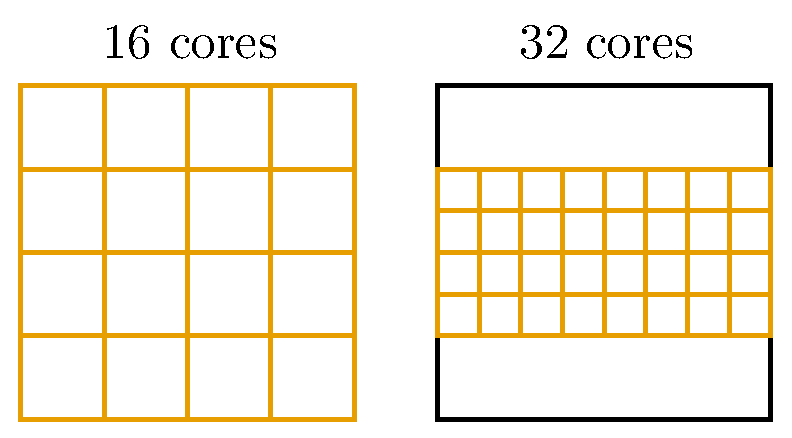
\includegraphics[width=0.3\linewidth]{include/revision/floorplans.pdf}
  \caption{16-core and 32-core floorplans.}
  \flabel{floorplans}
\end{figure}
For example, 16 cores form a four-by-four grid, a perfect square, whereas 32 cores form an eight-by-four grid, a rectangle.
Therefore, the processing elements in the first case cover the whole area of the die while the processing elements in the second case are concentrated along the middle line covering only half the area of the die, as shown in \fref{floorplans}.
As a result, the processing elements are closer to each other in the second floorplan, making it more favorable for model order reduction with respect to the squared-exponential kernel $\fCorr_\SE$ prioritized by $\eta = 1$.\footnote{As mentioned in the paper, all the floorplans used in our experiments are available online.}

\begin{actions}
  \action{The decrease of $\nvars$ has been noted and explained in Sec.~VII-B.}
\end{actions}
\end{authors}

\begin{reviewer}
\clabel{4}{5}
Why the reported error of 5.71\% for variance is likely to be overestimated? Even though the MC simulation with 10\^{}5 is not reliable (good enough), it does not mean that the report error of the developed framework is overestimated.
\end{reviewer}
\begin{authors}
The reviewer is right that there is no direct implication here, and we tried to emphasize a degree of our uncertainty using the word \emph{likely}.
Let us explain our reasoning.

In Tab.~III, we observe a drop of the error for variance from 9.80\% to 5.71\% for $10^4$ and $10^5$ samples, respectively.
The large gap of 4.09\% between the two values suggests that it is \emph{likely} that the next error change would \emph{not} be negligible if we could draw $10^6$ samples, for example.
Consequently, the reported error for variance is \emph{likely} to be overestimated, that is, the actual error is \emph{likely} to be smaller than the reported one of 5.71\%.

We agree that the sentence can indeed be confusing.

\begin{actions}
  \action{The sentence has been removed from Sec.~VII.}
\end{actions}
\end{authors}

\begin{reviewer}
\clabel{4}{6}
Could the authors explain how to decide the mapping matrix \textbackslash{}tilde\{B\} and why in Appendix A?
\end{reviewer}
\begin{authors}
Let us first recall that $\mM$ is an $\nnodes \times \nprocs$ matrix.
The purpose of this matrix is to relate $\nprocs$ processing elements with $\nnodes$ thermal nodes.
It can be thought of as a way to distribute the power dissipation of the processing elements across the thermal nodes.
If $\v{P} \in \real^\nprocs$ is a power vector with respect to the processing elements then $\v{P}' = \mM \, \v{P} \in \real^\nnodes$ is a power vector with respect to the thermal nodes.

The structure of $\mM$ depends on the way the equivalent thermal circuit is constructed.
For example, in the experimental results, the circuits follow the relation $\nnodes = 4 \, \nprocs + 12$, given in Sec.~VI-C.
One processing element is mapped onto one active thermal node, and $3 \, \nprocs + 12$ nodes are due to the thermal package, which does not dissipate power.
In this case, $\mM$ is filled in with zeros except for $\nprocs$ elements equal to unity that are located on the main diagonal of $\mM$ as shown below:
\[
  \mM = \left(
    \begin{array}{ccccc}
      1 & 0 & 0 & \cdots & 0 \\
      0 & 1 & 0 & \cdots & 0 \\
      0 & 0 & 1 & \cdots & 0 \\
      \vdots & \vdots & \vdots & \ddots & \vdots \\
      0 & 0 & 0 & \cdots & 1 \\
      0 & 0 & 0 & \cdots & 0 \\
      \vdots & \vdots & \vdots & \ddots & \vdots \\
      0 & 0 & 0 & \cdots & 0
    \end{array}
  \right).
\]
Then, the transpose of this matrix allows us to perform the reverse operation.
Namely, if $\v{Q}' \in \real^\nnodes$ is a temperature vector with respect to the thermal nodes then $\v{Q} = \mM^T \, \v{Q}' \in \real^\nprocs$ is a temperature vector with respect to the processing elements.

\begin{actions}
  \action{The structure of $\mM$ has been clarified in App.~A.}
\end{actions}
\end{authors}

\begin{reviewer}
\clabel{4}{7a}
The authors tried to use  ``(...)'' to help the readers to understand the work. However, it is getting kind of annoying if too many of them are used.
\end{reviewer}
\begin{authors}
We apologize for this inconvenience.
We were trying our best to make the paper transparent to as broad an audience as possible.
In the revised version of the manuscript, some of the explanations have been reformulated in order to avoid the use of parentheses.

\begin{actions}
  \action{The number of parentheses has been reduced.}
\end{actions}
\end{authors}

\begin{reviewer}
\clabel{4}{7b}
A typo: ``A description of the latter can also found in the supplementary materials, App. B'' (lines 26\~{}28, page 5).
\end{reviewer}
\begin{authors}
Thank you for pointing out the typo.

\begin{actions}
  \action{The typo found by the reviewer has been fixed in Sec.~V-A.}
\end{actions}
\end{authors}
